\documentclass[mat1]{fmfdelo}
\usepackage{graphicx}
\usepackage{amsmath}
\usepackage[shortlabels]{enumitem}
% \documentclass[fin1]{fmfdelo}
% \documentclass[isrm1]{fmfdelo}
% \documentclass[mat2]{fmfdelo}
% \documentclass[fin2]{fmfdelo}
% \documentclass[isrm2]{fmfdelo}

% naslednje ukaze ustrezno napolnite
\avtor{Matej Novoselec}

\naslov{Schwarzov princip zrcaljenja za harmonične funkcije}
\title{Schwarz Reflection Principle for Harmonic Functions}

% navedite ime mentorja s polnim nazivom: doc.~dr.~Ime Priimek,
% izr.~prof.~dr.~Ime Priimek, prof.~dr.~Ime Priimek
% uporabite le tisti ukaz/ukaze, ki je/so za vas ustrezni
\mentor{prof. dr. Barbara Drinovec Drnovšek}
% \mentorica{}
% \somentor{}
% \somentorica{}
% \mentorja{}{}
% \mentorici{}{}

\letnica{2023} % leto diplome

%  V povzetku na kratko opišite vsebinske rezultate dela. Sem ne sodi razlaga organizacije dela --
%  v katerem poglavju/razdelku je kaj, pač pa le opis vsebine.
\povzetek{}

%  Prevod slovenskega povzetka v angleščino.
\abstract{}

% navedite vsaj eno klasifikacijsko oznako --
% dostopne so na www.ams.org/mathscinet/msc/msc2020.html
\klasifikacija{}
\kljucnebesede{} % navedite nekaj ključnih pojmov, ki nastopajo v delu
\keywords{} % angleški prevod ključnih besed

\zapisiMetaPodatke  % poskrbi za metapodatke in veljaven PDF/A-1b standard

% aktivirajte pakete, ki jih potrebujete
% \usepackage{tikz}

% za številske množice uporabite naslednje simbole
\newcommand{\R}{\mathbb R}
\newcommand{\N}{\mathbb N}
\newcommand{\Z}{\mathbb Z}
\newcommand{\C}{\mathbb C}
\newcommand{\Q}{\mathbb Q}

% matematične operatorje deklarirajte kot take, da jih bo Latex pravilno stavil
% \DeclareMathOperator{\conv}{conv}

% vstavite svoje definicije ...
%  \newcommand{}{}

\begin{document}

\section{Uvod}
Znotraj diplomske naloge bomo spoznali osnovne lastnosti harmoničnih fukcij, ki jih bomo proti koncu s pridom uporabili za dokaz glavnega izreka, katerega ime nosi naslov naloge.
Ves čas se bomo opirali in vlekli številne vzporednice s kompleksno analizo. Gre za področje, močno povezano s študijo harmoničnih funkcij.
\newline
V prvem poglavju, bomo spoznali kaj so harmonične funkcije in poudarili, katere njihove lastnosti bodo za nadaljevanje pomembne. Ogledali si bomo tudi njihov odnos s holomorfnimi funkcijami. 
Znotraj drugega poglavja bomo spoznali Dirichletov problem za enostki disk, ki nam bo dal osnovo za definicijo Poissonovega jedra in Poissonovega integrala. Ogledali si bomo nekaj lastnosti obeh definiranih pojmov in z njuno pomočjo rešili na začetku poglavja zastavljen Dirichletov problem.
Tretje poglavje je namenjeno karakterizaciji harmoničnih funkcij s pomočjo lastnosti povprečne vrednosti in analizi pomembnosti te karakterizacije. 
V zadnjem poglavju, bomo s pomočjo orodij, spoznanih v prejšnih poglavjih, navedli in dokazali glavni izrek diplomskega dela - Schwarzov princip zrcaljenja za harmonične funkcije.
%\section*{Slovar strokovnih izrazov}
%
%\geslo{}{}
%\geslo{}{}

%------------------------------------------------------------
\newpage
\section{Harmonične funkcije}
    \begin{definicija}
        \label{harm}
        Funkcija $u(x_1, x_2, \dots, x_n)$ je \textbf{harmonična}, če velja
        $$
        \frac{\partial^2 u}{\partial x_1 ^ 2} +  \frac{\partial^2 u}{\partial x_2 ^ 2} + \dots + \frac{\partial^2 u}{\partial x_n ^ 2} = 0.
        $$
        Operatorju $\Delta  = \frac{\partial^2}{\partial x_1 ^ 2} +  \frac{\partial^2}{\partial x_2 ^ 2} + \dots + \frac{\partial^2}{\partial x_n ^ 2}$ pravimo Laplaceov operator in pišemo
        $$
        \Delta u = 0.
        $$
    \end{definicija}

    Pogoj za harmoničnost funkcije podaja (Laplaceovo) parcialno diferencialno enačbo, zapisano bodisi s Laplaceovim operatorjem ali razpisano s parcialnimi odvodi drugega reda. 
    Drugače rečeno, funkcija je harmonična, če zadošča zgoraj zapisani parcialni diferencialni enačbi. 
    Po tihem tu seveda privzemamo obstoj (vsaj) drugih parcialnih odvodov, saj drugače o harmoničnosti funkcije ne moremo govoriti.

    \begin{opomba}
        Vredno je omeniti, da nismo specificirali ali gre pri funkciji $u$ (harmoničnost katere bi radi opazovali) za realno ali kompleksno funkcijo. 
        Pojem harmoničnosti smo definirali v splošnem, torej tako za kompleksne, kot tudi realne funkcije.
        Znotraj diplomske naloge, se bomo omejili na funkcije dveh realnih spremenljivk ali funkcijo ene kompleksne spremenljivke, ki jo bomo nato delili na realni in imaginarni del ($z = x + iy $) in na ta način prešli nazaj na funkcije dveh realnih spremenljivk.
        \newline
        Pogoj za harmoničnost takrat zapišemo kot: 
            $$
                \Delta u = \frac{\partial^2 u}{\partial x ^ 2} +  \frac{\partial^2 u}{\partial y ^ 2}= 0.
            $$
    \end{opomba}
    \begin{trditev}
        \label{hh}
        Naj bo $f = u + iv$ holomorfna funkcija. Potem sta funkciji $u$ in $v$ harmonični. Rečeno drugače, realni in imaginarni del holomorfne sta harmonični funkciji. 
    \end{trditev}
    \begin{dokaz}
        Z uporabo Cauchy-Riemannovega sistema enačb lahko bralec sam hitro preveri, da trditev drži.
    \end{dokaz}

    \begin{definicija}
        Naj bo funkcija $u$ na območju $D$ harmonična. Če obstaja harmonična funkcija $v$, definirana na $D$, tako da je funkcija $f + u + iv$ na $D$ holomorfna, potem funkciji $v$ pravimo \textbf{harmonična konjugiranka funkcije $u$} (na $D$).    
    \end{definicija}

    \begin{trditev}
        \label{konj}
        Naj bo $u$ harmonična funkcija, definirana na zvezdastem območju $D$. Potem za $u$ na $D$ obstaja harmonična konjugiranka $v$ in je do konstante natančno enolično določena. 
    \end{trditev}
    \begin{dokaz}
        Konstrukcijo harmonične konjugiranke, si bralec za primer, ko je zvezdasto območje kar odprt disk lahko ogleda v \cite{osnova}. 
        Ideja dokaza v splošnem je podobna. 
    \end{dokaz}

    \begin{opomba}
        V duhu zgornjih dveh trditev, je velikokrat smiselno na harmonične funkcije gledati kot na realne dele holomorfnih funkcij. Prav to že nekako nakazuje, da se bodo vsaj nekatere "lepe/željene" lastnosti, ki jih holomorfne funkcije imajo, prenesle tudi na harmonične funkcije.
    \end{opomba}
    %%V duhu zgornjih dveh opomb, opazimo, da lahko kompleksno funkcijo $f$, zapišemo v obliki realnega in imaginarnega dela oziroma kot $f = u + i v$, s pomočjo nekih realnih funkcij (dveh spremenljivk) $u$ in $v$, ter lahko zaradi linearnosti parcialnih odvodov sklepamo, da je za harmoničnost $f$ kot kompleksne funkcije, dovolj zahtevati harmoničnost $u$ in $v$ kot realnih funkcij.
    %%Podoben argument nam da vedeti, da nam harmoničnost $f = u + iv$, implicira tudi harmoničnost $u$ in $v$. 
    \begin{opomba}
        \label{lin}
        Očitno, vendar le vredno spomniti, je da je zaradi linearnosti parcialnih odvodov tudi linearna kombinacija harmoničnih funkcij harmonična. To bomo pri reševanju enega izmed glavnih problemov diplomskega dela s pridom uporabili.
    \end{opomba}
    \begin{opomba}
        V literaturi se v definiciji harmoničnosti za funkcijo $u$ pojavlja tudi zahteva, da je funkcija gladka, oziroma $u \in C^{\infty}$. V zgornji definiciji zahtevamo le obstoj drugih parcialnih odvodov, oziroma $u \in C^2$. 
        Ekvivalentnost definicij potrdi spodnja trditev.
    \end{opomba}
    \begin{trditev}
        \label{gladkosth}
        Naj bo $u$ harmonična funkcija na območju $D$. Potem je $u$ na $D$ gladka oziroma $u \in C^{\infty}(D)$. 
    \end{trditev}
    \begin{dokaz}
        Za vsako točko $z \in D$, lahko najdemo dovolj majhno zvezdasto okolico $U_z$ (lahko kar dovolj majhen disk), tako, da bo okolica v celoti vsebova v $D$. 
        Po trditvi \ref{konj} na $U_z$ obstaja harmonična konjugiranka t.j. $v$, tako da je $f = u+ iv$ holomorfna na $U_z$. To pa že obstaja gladkost $u$ na $U_z$ oziroma gladkost v okolici poljubno izbrane točke iz $D$. 
    \end{dokaz}

\newpage
\section{Dirichletov problem za enotski disk}
    \begin{pro}
        Naj bo $\mathbb{D}$ enotski disk. Zvezno kompleksno funkcijo $h$, definirano na $\partial \mathbb{D}$, razširi do zvezne funkcije $\widetilde{h}$, tako da bo $\widetilde{h}$ harmonična na $\mathbb{D}$ in zvezna na $\overline{\mathbb{D}}$, ter se bo zožitev $\widetilde{h}$ na $\partial \mathbb{D}$ ujemala s $h$.
    \end{pro}

    \begin{opomba}
        Kot je bilo to že komentirano po definiciji \ref{harm}, so funkcije harmonične, natanko tedaj ko zadoščajo Laplaceovi parcialno diferencialni enačbi. 
        Vredno je omeniti, da lahko na Direchletov problem za enotski disk gledamo tudi iz stališča teorije diferencialnih enačb. Gre za problem iskanja funkcije, ki na notranjosti območja (v našem primeru kar notranjost enotskega diska), reši Laplaceovo diferencialno enačbo, ob robnem pogoju, ki ga določa v naprej podana funkcija na robu območja (v našem primeru začetna zvezna funkcija, podana na enotski krožnici). 
        Navadno se v teoriji parcialnih diferencialnih enačb srečamo s tako imenovanimi dobro postavljenimi matematičnimi problemi, o katerih si bralec več lahko prebere na REFERENCA. 
        Spodaj se bomo le seznanili z njihovo definicijo in pokazali, da zgoraj zastavljen Dirichletov problem ustreza definiciji. 
    \end{opomba}

    \begin{definicija}[J. Hadamard 1902]
        Pravimo, da je matematičen problem (parcialno diferencialnih enačb z robnimi in začetnimi pogoji) \textbf{dobro postavljen}, če zanj velja:
        \begin{itemize}
            \item rešitev problema obstaja,
            \item rešitev problema je ena sama, oziroma rešitev je enolično določena,
            \item rešitev je zvezno odvisna od začetnih podatkov problema.
        \end{itemize}
    \end{definicija}

    \begin{lema}
        \label{enolicno}
        Če rešitev za Dirichletov problem na enotskem disku obstaja, je enolično določena.
    \end{lema}
    \begin{dokaz}
        Denimo, da obstajata dve rešitvi Dirichletovega problema za enotski disk, $h_1$ in $h_2$.
        Oglejmo si razliko $h_1 - h_2$. Vemo, da je njuna razlika na $\partial \mathbb{D}$ enaka $0$, saj so njune vrednosti (kot rešitvi problema) enake vrednostim $h$. 
        Zaradi harmoničnosti $h_1$ in $h_2$ po principu o maksimu za harmonične funkcije vemo, da je njuna razlika ničelna tudi na $\mathbb{D}$. Sledi enakost $h_1$ in $h_2$ tudi na $\mathbb{D}$ in protislovje. 
    \end{dokaz}
    
    \begin{opomba}
        \label{op1}
        Po lemi \ref{enolicno}, opazimo, da je rešitev problema največ ena, zato se je dovolj posvetiti konstrukciji potencialne rešitve. 
        Opazimo, da lahko spremenljivko $z \in \partial \mathbb{D}$, funkcije $h$, zamenjamo z $e^{i \theta} \in \partial \mathbb{D}$, ter funkcijo $h(z)$ pišemo kot kompozitum $h(e^{i \theta})$.
        Poskusimo sedaj skonstruirati (harmonično) razširitev, ki bo zadoščala Dirichletovemu problemu za zvezno funkcijo $h(e^{i \theta})$.
    \end{opomba}

    \paragraph[short]{\textbf{Konstrukcija}}
    Kot velikokrat v matematiki, se najprej posvetimo enostavnim primerom in si nato teorijo oziroma konstrukcijo oglejmo v splošnem. 
    Naravno je za enostavne zvezne funkcije, definirane na $\partial \mathbb{D}$, vzeti kar polinome. V luči opombe \ref{op1} je polinomska spremenljivka lahko kar $e^{i\theta}$, s pomočjo opombe \ref{lin}, pa vidimo, da zadošča rešitve poiskati za posamezne faktorje polinoma, oziroma monome. 
    Zato si oglejmo funkcije oblike $h(e^{i \theta}) = e^{i k \theta}, k \in \mathbb{Z}$, ter za njih poskusimo skonstruirati željeno razširitev. 
    Brez večjih težav opazimo, da se nam v te primeru pojavlja preprosta eksplicitna razširitev s predpisom $\widetilde{h}(r e^{i \theta}) = r^{|k|}e^{i k \theta},~\text{za}~r\in [0, 1]~\text{in}~~\theta \in [0, 2\pi]$. 
    Tako predpisana razširitev je za $k \geq 0$ očitno harmonična na $\mathbb{D}$ ($r^k e^{ik\theta} = z^k$ je namreč celo holomorfna funkcija), pri $k < 0$ pa dobimo razširitev, ki v splošnem ni holomorfna, a kljub temu je harmonična ($r^{-k} e^{ik\theta} = \overline{z}^{-k}$, kar je monom v konjugirani spremenljivki, ki je harmoničen).
    Prav tako je za vsak $k \in \mathbb{D}$ razširitev očitno zvezna na $\overline{\mathbb{D}}$ in se na $\partial \mathbb{D}$ ujema z začetnimi pogoji (robnimi vrednosti podane funckije $h$), zato je res po lemi \ref{enolicno} enolična rešitev Dirichletovega problema. 
    Kot že omenjeno, lahko sedaj postopamo po linearnosti in za začetne funkcije oblike $h(e^{i\theta}) = \sum_{k = -N}^{N}{a_k e^{ik\theta}}$, konstruiramo razširitev s predpisom
    $\widetilde{h}(r e^{i \theta}) = \sum_{k = -N}^{N}{a_k r^{|k|}e^{ik\theta}}$. Smiselno bi bilo, predvsem v eksplicitnem predpisu razširitve, koeficiente $a_k$ izraziti direktno prek funkcije $h$. 
    V ta namen si oglejmo $\int_{-\pi}^{\pi}{e^{ij\theta} e^{-ik\theta}d\theta}$. S hitrim izračunom hitro preverimo tako imenovano ortogonalno relacijo med kompleksnimi eksponenti:
        $$
        \int_{-\pi}^{\pi}{e^{ij\theta} e^{-ik\theta}\frac{d\theta}{2\pi}} = 
        \begin{cases}
            1~&j=k\\
            0~&j \neq k\\
        \end{cases}
        .$$

        Zgornja relacija nam pri $h(e^{i\theta}) = \sum_{k = -N}^{N}{a_k e^{ik\theta}}$, omogoča izražavo koeficientov $a_k$ kot:
        $$
            a_ k = \int_{-\pi}^{\pi}{h(e^{i\theta}) e^{-ik\theta}\frac{d\theta}{2\pi}}.
        $$
    Sedaj lahko koeficiente izrazimo:
    $$
        \sum_{k = - N}^{N}{ a_k r^{|k|}e^{ik\theta}} = \sum_{k = - N}^{N} \bigg(\int_{-\pi}^{\pi}{h(e^{i \varphi}) e^{- i k \varphi} \frac{d \varphi}{2 \pi}}\bigg) r^{|k|} e^{i k \theta},
    $$
    zamenjamo vsoto in integral, ter brez škode iteracijsko območje vsote razširimo na vsa cela števila (pri dodanih indeksih je člen vsote ničeln). Dobimo željeni ekspliciten zapis:
    \begin{equation}
        \label{int1}
        \tag{P}
        \widetilde{h}(r e^{i \theta}) = \int_{-\pi}^{\pi}{h(e^{i \varphi}) \bigg[\sum_{k = - \infty}^{\infty} r^{|k|} e^{- i k \varphi} e^{i k \theta}} \bigg]\frac{d \varphi}{2 \pi}, ~~~ r e^{i\theta} \in \overline{\mathbb{D}}.
    \end{equation}
    Že iz načina konstrukcije in sprotnih komentarjev je jasno, da funkcija te oblike, za primere, ko je $h$ (trigonometričen) polinom reši Dirichletov problem.
    Sedaj bomo zgornjo funkcijo, ki smo jo na intuitiven način konstruirali s pomočjo začetnega pogoja preprostih zveznih funkcij $h$ (katere vrednosti poznamo na $\partial \mathbb{D}$) vzeli za definicijo novega pojma in z njegovo pomočjo prišli do rešitve/razširitve za splošno začetno zvezno funkcijo $h$.
    \begin{definicija}
        \textbf{Poissonovo jedro} je funkcija definirana s predpisom
        $$
           P_r(\theta) = \sum_{k = -\infty}^{\infty}{r^{|k|} e^{i k \theta}}\text{, kjer je}~\theta \in [-\pi, \pi]~\text{in}~ r < 1.
        $$
    \end{definicija}
    Na Poissonovo jedro lahko gledamo kot funkcijo dveh spremenljivk ($\theta$ in $r$) ali pa kot družino funkcij, indeksiranih s parametrom $r$.
    \newline
    Smiselno se je vprašati, ali je za vsako vrednost iz zapisanega definicijskega območje Poissonovega jedra vrsta na desni strani definicijske enakosti sploh konvergira. Potencialne strahove pomiri naslednja trditev.
    \begin{trditev}
        Za vsak fiksen $\rho < 1$, vrsta, definirana s Poissonovim jedrom konvergira enakomerno za vsak $r\leq \rho < 1$ in vsak $ -\pi \leq \theta \leq \pi$.
    \end{trditev}
    \begin{dokaz}
        Za vsak člen vrste velja $|r^{|k|} e^{i k \phi}| \leq \rho^{|k|}$, zato po Weierstrassovem M-testu velja, da vrsta konvergira enakomerno.
    \end{dokaz}

    Definicijo Poissonovega jedra, bi lahko ekvivalentno zapisali tudi kot:
        \begin{equation}
            \label{eq1}
            P_r(\theta) = 1 + \sum_{k=1}^{\infty}{z^k} + \sum_{j=1}^{\infty}{\overline{z}^{j}},~\text{kjer}~z = r e^{i\theta} \in \mathbb{D},~~~\text{oziroma}
        \end{equation}
        \begin{equation}
            \label{eq2}
            P_r(\theta) = \frac{1 - |z|^2}{|1-z|^2} = \frac{1-r^2}{1+ r^2 - 2r \cos(\theta)},~\text{kjer}~z= re^{i\theta} \in \mathbb{D}.
        \end{equation}
    Pokazati ekvivalentnost definicije z zapisom \ref{eq1} je dokaj trivialno, vrsto v definiciji le razbijemo na tri dele (glede na predznačenost iterativnega indeksa) in člen vsake izmed vsot zapišemo s kompleksno spremenljivko. 
    Za dokaz ekvivalence z drugo alternativno definicijo se moramo nekoliko bolj potruditi in pomagati z \ref{eq1}. Vrsti v \ref{eq1} sta definirani za notranjost enotskega diska (kjer je absolutna vrednost manjša od 1), zato obe vrsti konvergirata in ju lahko seštejemo s pomočjo formule za geometrijsko vrsto. 
    Prek enakosti $|1 - z|^2 = (\overline{1 - z})(1 - z) = (1 - \overline{z})(1 - z) = 1 + r^2 - 2r \cos(\theta)$ dobimo ekvivalenco z zapisom \ref{eq2}:
    $$
        P_r(\theta) = 1 + \frac{z}{1 - z} + \frac{\overline{z}}{1 - \overline{z}} = \frac{1 - |z|^2}{|1 - z|^2} = \frac{1 - r^2}{1 + r^2 - 2r\cos(\theta)}.
    $$
    Preden se lotimo uporabe novo definiranega pojma, si oglejmo še nekaj njegovih lastnosti. 
    
    \begin{trditev}
        \label{lastpk}
        Funkcija Poissonovega jedra ima naslednje lastnosti:
        \begin{enumerate}
            \item funkcija Poissonovega jedra je periodična s periodo $2\pi$, 
            \item za vsak fiksen $r \in [0,1): \int_{-\pi}^{\pi}{P_r(\theta) \frac{d\theta}{2\pi}} = 1$,
            \item za vsak fiksen $r \in [0,1)~\text{in}~-\pi \leq \theta \leq \pi: P_r(\theta) > 0$,
            \item za vsak fiksen $r \in [0,1)~\text{in}~-\pi \leq \theta \leq \pi: P_r( - \theta) = P_r(\theta)$,
            \item za vsak fiksen $r \in [0,1): P_r(\theta)~\text{na}~-\pi \leq \theta \leq 0~\text{narašča in na}~0 \leq \theta \leq \pi~\text{pada}$,
            \item za vsak fiksen $\delta > 0: \text{max}\{P_r(\theta)~|~ \delta \leq |\theta| \leq \pi\} \to 0$ ko gre $r \to 1$,
            \item Poissonovo jedro je kot funkcija dveh spremenljivk ($r$ in $\theta$) harmonična.
        \end{enumerate}
    \end{trditev}
    \begin{dokaz}
        $ $
        \begin{enumerate}
            \item Periodičnost funkcije, s periodo $2\pi$, je zaradi definiranosti prek vsote členov $e^{ik\theta}$ očitna. 
            \item Oglejmo si \ref{int1} in vzemimo $h \equiv 1$. Dobimo: 
            $$
                \widetilde{h}(r e^{i \theta}) = \int_{-\pi}^{\pi}{\bigg[\sum_{k=-\infty}^{\infty}{r^{|k|} e^{ik(\varphi - \theta)}}\bigg] \frac{d \varphi}{2 \pi}} = \int_{-\pi}^{\pi}{P_r(\varphi - \theta)\frac{d \varphi}{2 \pi}}. 
            $$
            Opazimo, da $\widetilde{h} \equiv 1$ reši Dirichletov problem, zato je po lemi \ref{enolicno} edina rešitev. Uporabimo translacijo $\varphi \mapsto \varphi - \theta$ za uvedbo nove spremenljivke v integral, ter ob upoštevanju periodičnosti dobimo:
            $$
                1 = \int_{-\pi}^{\pi}{P_r(\varphi - \theta)\frac{d \varphi}{2 \pi}} = \int_{-\pi}^{\pi}{P_r(\varphi)\frac{d \varphi}{2 \pi}}.
            $$
            \item Trditev očitno sledi iz definicije \ref{eq2}. 
            \item Trditev očitno sledi iz definicije \ref{eq2}. 
            \item Trditev očitno sledi iz definicije \ref{eq2}. 
            \item TODO 
            \item Po trditvi \ref{hh} zadošča pokazati, da lahko Poissonovo jedro zapišemo kot realni del holomorfne funkcije (definirane na $\mathbb{D}$). Opazimo, da po \ref{eq1} to res lahko storimo kot:
            $$
                P_r(\theta) = 1 + 2~\text{Re}\bigg(\frac{z}{1-z}\bigg) = \text{Re}\bigg(\frac{1+z}{1-z}\bigg),~\text{za}~z= re^{i\theta} \in \mathbb{D}.
            $$
        \end{enumerate}
    \end{dokaz}
    \begin{opomba}
        Lastnosti Poissonovega jedra, navedene v trditvi \ref{lastpk}, so tudi dobro razvidne na spodnji sliki. 
        \newline
        SLIKA - GRAF POISSONOVEGA JEDRA
        \newline
        Vredno je omeniti tudi, da točki (2) in (3) trditve \ref{lastpk} nakazujeta, da funkcija $\frac{1}{2 \pi} P_r(\theta)$ določa gostoto zvezno porazdeljene slučajne spremenljivke.
    \end{opomba}
    Sedaj se vrnimo k reševanju Dirichletovega problema za enotski disk. 
    Spomnimo se, da smo za polinomske funkcije $h$ skonstruirali predpis razširitve, ki je rešila zastavljen problem. 
    Opazimo, da si sedaj lahko pomagamo z definiranim pojmom Poissonovega jedra in zapišimo:
    $$
    \widetilde{h}(r e^{i \theta}) = \int_{-\pi}^{\pi}{h(e^{i \varphi}) \bigg[\sum_{k = - \infty}^{\infty} r^{|k|} e^{- i k \varphi} e^{i k \theta}} \bigg]\frac{d \varphi}{2 \pi} = 
    \int_{-\pi}^{\pi}{h(e^{i \varphi}) P_r(\theta - \varphi)\frac{d \varphi}{2 \pi}}.
    $$
    Če (trigonometričen) polinom $h(e^{i\theta})$ (ki  bi seveda lahko zavzemal kompleksne vrednosti), zamenjamo s (trigonometričnim) polinomom $u(e^{i\theta})$, ki zavzema le realne vrednosti, se nam zgornja enakost v duhu 
    točke (7) trditve \ref{lastpk}, še olepša. Takrat lahko namreč za $z = re^{i\theta} \in \mathbb{D}$ pišemo:
    \begin{equation}
        \label{realnidel}
        \begin{split}
            \widetilde{u}(z) = \widetilde{u}(r e^{i \theta}) = \int_{-\pi}^{\pi}{u(e^{i \varphi}) P_r(\theta - \varphi)\frac{d \varphi}{2 \pi}} = \int_{-\pi}^{\pi}{u(e^{i \varphi})~\text{Re}\bigg(\frac{1+re^{i(\theta - \varphi)}}{1-re^{i(\theta - \varphi)}}\bigg)\frac{d \varphi}{2 \pi}}= \\
            \int_{-\pi}^{\pi}{u(e^{i \varphi})~\text{Re}\bigg(\frac{e^{i\varphi}+re^{i\theta}}{e^{i\varphi}-re^{i\theta}}\bigg)\frac{d \varphi}{2 \pi}}=~\text{Re}~\bigg[\int_{-\pi}^{\pi}{u(e^{i \varphi})\bigg(\frac{e^{i\varphi}+z}{e^{i\varphi}-z}\bigg)\frac{d \varphi}{2 \pi}}\bigg].
        \end{split}
    \end{equation}
    Opazimo, da nam je uspelo $\widetilde{u}(z)$ za $z \in \mathbb{D}$ izraziti kot realni del holomorfne funkcije, ne le implicira harmoničnost predpisa (po trditvi \ref{hh}) ampak tudi gladko odvisnost $\widetilde{u}(z)$ od spremenljivke/parametra $z$.
    \newline
    Posvetimo se sedaj nazaj iskanju splošne rešitve Dirichletovega problema. Zgoraj smo z intuitivno izpeljavo nevede že zapisali funkcijo, ki jo bomo sedaj vzeli za definicijo novega pojma, ter pokazali da tudi v splošnem pripelje do rešitve.

    \begin{definicija}
        \textbf{Poissonov integral}, ki ga označimo z~$\widetilde{h}(z)$, od zvezne funkcije $h(e^{i\theta})$ je funkcija, definirana na enotskem disku s predpisom
        $$
        \widetilde{h}(z) = \int_{-\pi}^{\pi}{h(e^{i\varphi}) P_r(\theta - \varphi)~\frac{d\varphi}{2 \pi}}~\text{, kjer}~~z = r e^{i\theta} \in \mathbb{D}.
        $$
     \end{definicija}
     \begin{opomba}
        Ekvivalentno bi lahko definicijo Poissonovega integrala, zaradi ($2\pi$) periodičnosti Poissonovega jedra,  zapisali tudi kot:
        $$
        \widetilde{h}(z) = \int_{-\pi}^{\pi}{h\big(e^{i(\theta-\varphi)}\big) P_r(\varphi)~\frac{d\varphi}{2 \pi}}~\text{, kjer}~~z = r e^{i\theta} \in \mathbb{D}.
        $$
     \end{opomba}
     \begin{trditev}
        \label{lastpi}
        Za  preslikavo $\Phi : h \mapsto \widetilde{h}$, t.j. preslikavo, ki  zvezni funkciji $h$, definirani na $\partial \mathbb{D}$ priredi njen Poissonov integral, velja:
        \begin{enumerate}
            \item $\Phi$ je linearna preslikava, t.j. $\Phi(c_1 h_1 + c_2 h_2) = c_1 \widetilde{h_1} + c_2 \widetilde{h_2}$,
            \item $\Phi$ "ohranja omejenost", t.j. če $|h| \leq M$ na $\partial \mathbb{D}$, potem $|\widetilde{h}| \leq M$ na $\mathbb{D}$.
        \end{enumerate}
     \end{trditev}
     \begin{dokaz}
        $ $
        \begin{enumerate}
            \item Trditev trivialno sledi iz definicije Poissonovega integrala, zaradi linearnosti integrala. 
            \item Trditev sledi iz točke (2) in (3) trditve \ref{lastpk}.
        \end{enumerate}
     \end{dokaz}
        


     \begin{trditev}
        \label{obstoj}
        Naj bo $h$ zvezna kompleksna funkcija definirana na $\partial \mathbb{D}$. Rešitev Dirichletovega problema obstaja in ima vrednosti na $\mathbb{D}$ definirane kot Poissonov integral funkcije $h$.
        \newline
        Rečeno drugače, Poissonov integral zvezne kompleksne funkcije, definirane na $\partial \mathbb{D}$ je zvezna harmonična funkcija, definirana na $\mathbb{D}$, ki nam ponuja zvezno harmonično razširitev $h$ na $\overline{\mathbb{D}}$, če jo dodefiniramo na $\mathbb{D}$ z njenim Poissonovim integralom.
     \end{trditev}
     \begin{dokaz}
        Trditev dokaži v dveh korakih. Najprej dokažimo, da je Poissonov integral na $\mathbb{D}$ harmonična funkcija.
        Vemo, da lahko vsako kompleksno funkcijo $h$ zapišemo/razcepimo na njen realni in imaginarni del kot $h = u + iv$, pri čemer sta $u$ in $v$ funkciji (ene kompleksne ali dveh realni spremenljivk), z zalogo vrednostjo znotraj realnih števil. 
        Zaradi linearnosti Poissonovega integrala, po trditvi \ref{lastpi} se lahko sedaj posebej skoncentriramo na Poissonov integral realnega ($\widetilde{u}$) in Poissonov integral imaginarnega ($\widetilde{v}$) dela. 
        Tako, kot smo to naredili pri \ref{realnidel}, lahko vsakega izmed Poissonovih integralov $\widetilde{u}$ in $\widetilde{v}$ zapišemo kot realni del neke holomorfne funkcije, kar nam po trditvi \ref{hh} implicira harmoničnost $\widetilde{u}$ in $\widetilde{v}$.
        Zaradi opombe \ref{lin}, nam to implicira tudi harmoničnost $\widetilde{h} = \widetilde{u} + i\widetilde{v}$, ter dokaz prvega dela trditve. 
        \newline
        Za dokaz zveznosti na $\overline{\mathbb{D}}$ se moramo nekoliko bolj potruditi. Uporabili bomo lastnosti Poissonovega jedra iz trditve \ref{lastpk}. 
        Ker je $h$ na $\partial \mathbb{D}$ zvezna, je kot zvezna funkcija na kompaktu: 
        \begin{itemize}
            \item omejena, t.j.:$~\exists M: |h(e^{i\theta})| \leq M$ in 
            \item enakomerno zvezna, t.j.: $\forall \epsilon > 0, \exists \delta > 0: | \theta - \varphi | < \delta \Rightarrow |h(e^{i\theta}) - h(e^{i\varphi})| < \epsilon $.
        \end{itemize}
        Po točki (2) iz trditve \ref{lastpk}, lahko zapišemo:
        $$
            \widetilde{h}(re^{i\theta}) - h(e^{i\theta}) = \int_{-\pi}^{\pi}{\bigg[h\big(e^{i(\theta - \varphi)}\big) - h(e^{i\theta})\bigg]P_r(\theta)\frac{d\varphi}{2\pi}}.
        $$
        Sedaj vzamemo absolutno vrednost leve in desne strani enakosti, ter uporabimo trikotniško neenakost. Dobimo:
        $$
        |\widetilde{h}(re^{i\theta}) - h(e^{i\theta})| \leq \int_{-\pi}^{\pi}{\bigg| h\big(e^{i(\theta - \varphi)}\big) - h(e^{i\theta})\bigg|P_r(\theta)\frac{d\varphi}{2\pi}}.
        $$
        Integral lahko razdelimo na dva dela, tako, da bomo lahko uporabili enakomerno zveznost funkcije:
        $$
        |\widetilde{h}(re^{i\theta}) - h(e^{i\theta})| \leq \bigg(\int_{-\delta}^{\delta} + \int_{\delta \leq |\varphi| \le \pi}\bigg){\bigg| h\big(e^{i(\theta - \varphi)}\big) - h(e^{i\theta})\bigg|P_r(\theta)\frac{d\varphi}{2\pi}}.
        $$
        Vrednosti znotraj prvega integral lahko zaradi enakomerne zveznosti navzgor ocenimo z $\epsilon$, vrednosti znotraj drugega integrala, pa lahko prek omejenosti navzgor ocenimo kar z $2M$. 
        $$
        |\widetilde{h}(re^{i\theta}) - h(e^{i\theta})| \leq \epsilon \int_{-\delta}^{\delta}{P_r(\theta) \frac{d\varphi}{2\pi}} + 2M\int_{\delta \leq |\varphi| \leq \pi}{P_r(\theta)\frac{d\varphi}{2\pi}}.
        $$
        Vsakega od integralov lahko sedaj v duhu točke (2) trditve \ref{lastpk} navzgor ocenimo in dobimo:
        $$
        |\widetilde{h}(re^{i\theta}) - h(e^{i\theta})| \leq \epsilon  + 2M~\text{max}\{P_r(\varphi)~| ~\delta \leq |\varphi| \leq \pi \}.
        $$
        Sedaj uporabimo točko (6) trditve \ref{lastpk}, ki nam pove, da gre drugi sumand res proti 0, ko gre $r$ proti 1. 
        Torej, za vsak $\widetilde{\epsilon} > 0$, pri $r$, ki je dovolj blizu 1, velja, da $|\widetilde{h}(re^{i\theta}) - h(e^{i\theta})| < \widetilde{\epsilon}$.
        Zveznost in trditev je s tem dokazana.
    \end{dokaz}
    \begin{posledica}
        Dirichletov problem za enotski disk, je dobro postavljen matematičen problem. 
    \end{posledica}
    \begin{dokaz}
        Obstoj rešitve za vsako zvezno začetno podano funkcijo, nam (eksplicitno) zagotavlja trditev \ref{obstoj}. 
        Enoličnost rešitve, nam zaradi že zagotovoljenega obstoja zagotavlja lema \ref{enolicno}, zvezna odvisnost rešitve od začetnih podatkov, pa je predpostavka problema (funkcija reši problem le v primeru, ko je zvezna na zaprtju enotskega diska, kar nam zagotavlja zvezno odvisnost od pogojev na robu diska oziroma zvezno odvisnost od začetnih pogojev).
    \end{dokaz}
    \begin{opomba}
        \label{alldisk}
        Dirichletov problem smo formulirali in reševali za enotski disk. Problem bi na podoben način lahko formulirali za poljubno območje $U$. 
        Kot začetni/robni pogoj bi podali zvezno funckijo $f$ (definirano na $\partial U$), ter iskali njeno razširitev $\widetilde{f}$ (na $\overline{U}$), tako da bi bila na $\overline{U}$ zvezna, 
        na $U$ harmonična, ter bi se zožitev $\widetilde{f}$ na $\partial U$ ujemala z $f$.
        V splošnem Dirichletovega problema znotraj diplomske naloge ne bomo reševali, vredno pa je omeniti, 
        da je bil prav enotski disk izbran zaradi preprostosti in bi lahko zgornji rezultat na podoben način zapisali za poljuben disk. To naredimo s pomočjo vpeljave novih spremenljivk ($z \to az + b$) v Poissonov integral. 
        DOKONCAJ IZPELJAVO!
     \end{opomba}

\newpage
\section{Lastnost povprečne vrednosti}

    \begin{definicija}  
        Naj bo $h$ zvezna funkcija na območju $D$. Denimo, da za $z_0 \in D$ in $r$ velja  $\overline{\mathbb{D}}(z_0, r) \subseteq D$. \textbf{Povprečje funkcije} $h$ na $\overline{\mathbb{D}}(z_0, r)$ definiramo kot:
        $$
            A(r) = \int_{0}^{2 \pi}{h \big(z_0 + r e^{i\theta}\big)\frac{d\theta}{2 \pi}}.
        $$
    \end{definicija}
    \begin{trditev}
        \label{zvpov}
        Naj bo $h$ zvezna funkcija, definirana na območju $D$. Naj bo $\overline{\mathbb{D}}(z_0, r) \subseteq D$. 
        Potem je $A(r)$ zvezno odvisna od $r$ in velja: $\lim_{r \to 0}{A(r)} = h(z_0)$.
    \end{trditev}
    \begin{dokaz}
        $A(r)$ je zvezno odvisna od $r$, saj je definirana kot integral zvezne funkcije. Drugi del trditve nam dokaže:
        $$
            |A(r) - h(z_0)| = \bigg|\int_{0}^{2\pi} \big[h(z_0 + r e^{i\theta})  - h(z_0)\big] \frac{d\theta}{2\pi} \bigg| \leq \int_{0}^{2 \pi} \big| h(z_0 + r e^{i\theta}) - h(z_0) \big| \frac{d\theta}{2 \pi},
        $$
        saj lahko zaradi zveznosti $h$ notranjost integrala navzgor ocenimo s poljubno majhnim $\epsilon$ (pri dovolj majhnem $r$) in s tem dobimo $|A(r) - h(z_0)| < \epsilon$, za poljubno majhen $\epsilon$. 
    \end{dokaz}

    \begin{definicija}
        Zvezna funkcija $h$, definirana na območju $D \subseteq \C$ ima \textbf{lastnost povprečne vrednosti}, če za vsak $z_0 \in D$ obstaja $\epsilon_0 > 0$, da $\overline{\mathbb{D}}(z_0, \epsilon_0) \subseteq D$ in za vsak $0 < \epsilon \leq \epsilon_0 $ velja:
        $$
            h(z_0) = \frac{1}{2 \pi} \int_{0}^{2 \pi}{h(z_0 + \epsilon e^{i \theta}) d\theta}.
        $$
    \end{definicija}
    \begin{opomba}
        Definicija nam pove, da ima zvezna funkcija $h$, definirana na območju $D \subseteq \C$, lastnost povprečne vrednosti, če za vsak $z_0$ iz $D$ velja, 
        da je $h(z_0)$ povprečje vrednosti $h(z)$, kjer $z$ teče po majhni krožnici s središčem v $z_0$.
    \end{opomba}
    \begin{trditev}
        \label{linlpv}
        Linearna kombinacija funkcij s lastnostjo povprečne vrednosti, je funkcija z lastnostjo povprečne vrednosti. 
    \end{trditev}
    \begin{dokaz}
        Trditev sledi iz linearnosti integrala, prek katerega je definirana lastnost povprečne vrednosti.
    \end{dokaz}

    \begin{trditev}
        Naj bo $f$ holomorfna na območju $D$. Potem ima lastnost povprečne vrednosti.
    \end{trditev}
    \begin{dokaz}
        Predpostavka, da ja $f$ holomorfna nam omogoča uporabo Cauchyjeve integralske formule za vsak zaprt disk, ki je v celoti vsebovan v $D$. Torej za $z \in D$ in vsak $r$, tako da $\overline{\mathbb{D}}(z,r) \subseteq \mathbb{D}$ velja:
        $$
        f(z) = \frac{1}{2 \pi i} \int_{\partial \overline{\mathbb{D}}(z, r)}{\frac{f(\xi)}{\xi  - z}}d\xi.
        $$
        Ko rob diska parametriziramo, dobimo:
        $$
        f(z) = \frac{1}{2 \pi} \int_{0}^{2\pi}{f(z + re^{i\varphi})}d\varphi.
        $$
    \end{dokaz}

    \begin{trditev}
        \label{harmonicnapovp}
        Naj bo $u$ harmonična funkcija na območju $D \subseteq \C$. Za $z_0$ in $\rho$, kjer $\overline{\mathbb{D}}(z_0, \rho) \subseteq D$, velja:
            $$
                u(z_0) = \frac{1}{2 \pi} \int_{0}^{2 \pi}{u(z_0 + r e^{i \theta}) d\theta},~~\text{kjer}~~ 0 < r < \rho.
            $$
    \end{trditev}
    \begin{dokaz}
        Na $\overline{\mathbb{D}}(z_0, \rho) \subseteq D$ lahko za $P = -\frac{\partial u}{\partial y}$ in $Q = \frac{\partial u}{\partial x}$ uporabimo Greenovo integralsko formulo:
        $$
            \int_{\partial \overline{\mathbb{D}}(z_0, \rho)}{P dx + Q dy} = \iint_{\overline{\mathbb{D}}(z_0, \rho)}{\bigg(\frac{\partial Q}{\partial x} - \frac{\partial P}{\partial y}\bigg)dx dy}.
        $$ 
        Sedaj upoštevajmo pogoj za harmoničnost $u$ \big($\frac{\partial^2 u}{\partial x^2} + \frac{\partial^2 u}{\partial y^2} = 0$\big) in ga vstavimo v Greenovo formulo:
        $$
        \int_{\partial \overline{\mathbb{D}}(z_0, \rho)}{-\frac{\partial u}{\partial y} dx + \frac{\partial u}{\partial x} dy} = \iint_{\overline{\mathbb{D}}(z_0, \rho)}{\bigg(\frac{\partial^2 u}{\partial x^2} + \frac{\partial^2 u}{\partial y^2}\bigg)dx dy} = 0. 
        $$
        Rob diska lahko pri $z_0 = x_0 + iy_0$ parametriziramo z $x(\theta) = x_0 + \rho \cos(\theta),~y(\theta) = y_0 + \rho \sin(\theta)$. Ko to vstavimo v zgornjo enakost dobimo:
        $$
        0 = \rho \int_{0}^{2 \pi}{\bigg[\frac{\partial u}{\partial x} \cos(\theta) + \frac{\partial u}{\partial y} \sin(\theta)\bigg] d\theta} = \rho \int_{0}^{2\pi}{\frac{\partial u}{\partial \rho}\big({z_0 + \rho e^{i\theta}\big)d\theta}}.
        $$
        Ker je $u$ harmonična, je gladka, zato lahko zamenjamo limitna procesa integriranja in odvajanja, delimo z $2\pi \rho$ in zapišemo:
        $$
        0 = \frac{\partial}{\partial \rho} \int_{0}^{2\pi}{u\big({z_0 + \rho e^{i\theta}\big)\frac{d\theta}{2 \pi}}}.
        $$
        Sledi, da je vrednost zgornjega integrala konstanta, za vsak $0 <r < \rho$ t.j.: 
        $$
        \int_{0}^{2\pi}{u\big({z_0 + r e^{i\theta}\big)\frac{d\theta}{2 \pi}}} = c \in \mathbb{C},~ 0 < r < \rho.
        $$
        Opazimo, da je potrebno le še pokazati, da $c = u(z_0)$.
        Ker je $u$ zvezna, po trditvi \ref{zvpov} velja, da ko pošljemo $r \to 0$ dobimo:
        $$
        c = \lim_{r \to 0}{\bigg[\int_{0}^{2\pi}{u\big({z_0 + r e^{i\theta}\big)\frac{d\theta}{2 \pi}}}\bigg]} = \int_{0}^{2\pi}{{u(z_0)\frac{d\theta}{2 \pi}}} = u(z_0).
        $$
    \end{dokaz}
    \begin{opomba}
        Komentirali smo že, da imajo holomorfne funkcije lastnost povprečne vrednosti, zgornja trditev pa nam pove, da imajo lastnost povprečne vrednosti tudi harmonične funkcije. 
        Za harmonične funkcije velja celo več, da se jih namreč karakterizirati s pomočjo lastnosti povprečne vrednosti. 
    \end{opomba}
    \begin{trditev}
        \label{ekvhlp}
        Naj bo $h$ zvezna funkcija, definirana na območju $U \subseteq \C$. Velja, da je $h$ harmonična funkcija, natanko tedaj, ko ima lastnost povprečne vrednosti.
    \end{trditev}
    \begin{dokaz}
        Trditev \ref{harmonicnapovp} nam dokaže eno implikacijo. Dovolj je torej preveriti, da je zvezna funkcija $h$, z lastnostjo povprečne vrednosti na $U$ harmonična. 
        Dokaz temelji na že dokazanem obstoju rešitve Dirichletovega problema za enotski disk oziroma po opombi \ref{alldisk} obstoju rešitve Dirichletovega problema za poljuben disk. 
        \newline
        Ker je $U$ območje, za poljubno točko $z_0 \in U$ obstaja $r$, tako da $\overline{\mathbb{D}}(z_0,r) \subseteq U$. Ker je $h$ zvezna na $U$, $h$ na $\partial \overline{\mathbb{D}}(z_0, r)$ določa robne/začetne pogoje za Dirichletov problem za disk $\mathbb{D}(z_0,r)$.
        Vemo, da rešitev (označimo jo z $\widetilde{h}$) obstaja. 
        Kot harmonična funkcija, ima po trditvi \ref{harmonicnapovp} na $\mathbb{D}(z_0, r)$ lastnost povprečne vrednosti. 
        Oglejmo si sedaj funkcijo $g(z) = h(z) - \widetilde{z}$, za $z \in \overline{\mathbb{D}}(z_0,r)$. 
        Kot razlika funkcij s lastnostjo povprečne vrednosti, ima po trditvi \ref{linlpv} tudi $g$ na $\mathbb{D}(z_0, r)$ lastnost povprečne vrednosti in je kot razlika dveh zveznih funkcij, zvezna na $\overline{D}(z_0, r)$.
        Vemo celo, da na $\partial \overline{\mathbb{D}}(z_0, r)$ velja $g \equiv 0$, saj je zožitev $\widetilde{h}$ na $\partial \overline{\mathbb{D}}(z_0,r)$ enaka $h$. 
        Po principu maksima, za funkcije z lastnostjo povprečne vrednosti, je potem $g \equiv 0$ oziroma $\widetilde{h} \equiv h$ na $\overline{\mathbb{D}}(z_0, r)$, kar nam da harmoničnost $h$ na $\mathbb{D}(z_0, r)$. 
        Dokazali smo torej, da za poljubno točko $z_0 \in U$ obstaja disk, katerega zaprtje je vsebovano v $U$ in na notranjosti katerega je $h$ harmonična. To pa nam že zagotavlja harmoničnost $h$ na $U$. 
    \end{dokaz}
    \begin{trditev}
        Naj bo $u$ zvezna funkcija z lastnostjo povprečne vrednosti, definirana na območju $D$. Potem je $u$ na $D$ gladka oziroma $u \in C^{\infty}(D)$.
    \end{trditev}
    \begin{dokaz}
        Po trditvi \ref{ekvhlp} je $u$ harmonična, po trditvi \ref{gladkosth} pa zato tudi gladka.
    \end{dokaz}

\newpage
\section{Schwarzov princip zrcaljenja za harmonične funkcije}
    Znotraj tretjega poglavja, smo se že srečali s problemom razširitve podane funkcije, do funkcije, ki mora zahtevati dodatnim pogojem. 
    Pri Dirichletovem problemu smo tako zahtevali harmoničnost razširitve na notranjosti območja/diska in zveznost razširitve na zaprtju območja/diska. 
    Pokazali smo, da to lahko naredimo s pomočjo Poissonovega integrala $\widetilde{h}$ kot:
    $$
        h^e(z) = 
        \begin{cases}
            h(z)~&z \in \partial \mathbb{D} \\
            \widetilde{h}(z)~&z \in \mathbb{D}
        \end{cases}.
    $$
    Problem, ki ga Schwarzov princip zrcaljenja reši, je ne glede na drugačne začetne pogoje, v svojem bistvu iz vidika iskanja razširitve kljub temu blizu že rešenemu Dirichletovemu problemu.
    Glavna razlika je, da pri Schwarzovem principu zrcaljenja harmoničnost na območju vzamemo že za predpostavko, (ter s pomočjo robnih zveznih začetnih pogojev) poskušamo konstruirati harmonično razširitev na povsem novem območju, podobne oblike.  
    Kot to že nakazuje beseda zrcaljanje v imenu principa, bomo razširitev želeli konstruirati na "zrcalni sliki" prvotno definiranega območja. Prav zato bo potrebno predpostaviti nekaj simetrije.
    Spoznajmo sedaj nekaj osnovnih pojmov, ki nas bodo pripeljali do glavnega izreka.
    \begin{definicija}
        Naj bo $U$ območje. \textbf{Zrcaljenje območja U čez realno os} definiramo kot: $U^* = \{\overline{z}~|~z \in U\}$.
        \newline
        Pravimo, da je \textbf{območje U simetrično glede na realno os} če velja: $U^* = U$.
        \newline
        Naj bo $u: U \to \mathbb{R}$. Potem lahko pri zgornjih oznakah definiramo: $u^*: U^* \to \mathbb{R}$, kot $u^*(z) = u(\overline{z})$.
    \end{definicija}

    Naravno je pričakovati, da se zaradi dokaj preproste definicije $u^*$ prek $u$ lastnosti $u$ "prenesejo" tudi na $u^*$. 
    Spodnja lema nam to potrdi.

    \begin{lema}
        \label{lemaharm}
        Naj bo $U$ območje in $u: U \to \mathbb{R}$. Če je $u$ harmonična na $U$, je $u^*$ harmonična na $U^*$. 
    \end{lema}
    \begin{proof}
        Trditev lahko dokažemo na dva načina. Dokažimo najprej s pomočjo karakterizacije harmoničnih funkcij z lastnostjo povprečne vrednosti. 
        Ker je $u$ na $U$ harmonična ima na $U$ lastnost povprečne vrednosti.
        Sedaj je hitro jasno, da ima lastnost povprečne vrednosti tudi $u^*$ na $U^*$. 
        Iz trditve \ref{ekvhlp} potem sledi, da je $u^*$ na $U^*$ tudi harmonična.
        \newline
        Trditev je možno dokazati tudi kar direktno po definiciji t.j. dokazati, da velja: $\frac{\partial^2 u^*}{\partial x^2} + \frac{\partial^2 u^*}{\partial y^2} = 0$. 
        Opazimo, da lahko $u^*$ (s pomočjo identifikacije $z = x + iy \leftrightarrow (x,y)$) zapišemo tudi kot kompozitum $u \circ ((x,y) \mapsto (x, -y))$. 
        Sedaj po definiciji parcialno odvajamo in dobimo enakosti:
        $$
            \frac{\partial u^*}{\partial y} = - \frac{\partial u }{\partial y},~~~~\frac{\partial^2 u^*}{\partial y^2} = \frac{\partial^2 u }{\partial y^2},~~~~\frac{\partial^2 u^*}{\partial x^2} = \frac{\partial^2 u }{\partial x^2},
        $$
        ki implicirajo:
        $$
            \frac{\partial^2 u^*}{\partial x^2} + \frac{\partial^2 u^*}{\partial y^2} = \frac{\partial^2 u}{\partial x^2} + \frac{\partial^2 u}{\partial y^2} = 0.
        $$
    \end{proof}
    \begin{lema}
        Če je $f$ holomorfna na območju $U$ je $g(z) = \overline{f({\overline{z}})}$ holomorfna na $U^*$.
    \end{lema}
    \begin{dokaz}
        Iz kompleksne analize vemo, da je dovolj pokazati, da tudi $g$ zadošča Cauchy-Riemannovemu sistemu enačb.
        \newline
        Pišimo: $f(z) = u(z) + iv(z)$ in $g(z) = p(z) + iq(z)$.
        Potem je $g(z) = u(\overline{z}) - iv(\overline{z})$ in zato $p(z) = u(\overline{z}),\text{ter}~q(z) = -v(\overline{z})$. 
        \newline
        Velja:
        \begin{equation*}
            \frac{\partial p}{\partial x} = \frac{\partial u}{\partial x} \overset{C-R}{=} \frac{\partial v}{\partial y} = - \bigg(- \frac{\partial q}{\partial y}\bigg) = \frac{\partial q}{\partial y}~~~\text{in}~~~
            \frac{\partial p}{\partial y} = -\frac{\partial u}{\partial y} \overset{C-R}{=} \frac{\partial v}{\partial x} = -\frac{\partial q}{\partial x}.
        \end{equation*}
        Alternativen dokaz, si bralec lahko ogleda v REFERENCA.
    \end{dokaz}

    Sedaj smo pripravljeni na formulacijo in dokaz glavnega izreka.
    \begin{izrek}
        Naj bo $D \subseteq \C$ območje, simetrično glede na realno os. 
        Označimo $D^{+} = D \cap \{\text{Im} > 0\}$ in $D^{-} = D \cap \{\text{Im} < 0\}$.
        \newline
        Naj bo $u(z): D^{+} \to \mathbb{R}$ harmonična funkcija, za katero velja, da gre $u(z) \to 0$, ko gre $z \in D^{+}$ proti poljubni točki $D \cap \mathbb{R}$ t.j.: $$\lim_{\text{Im}(z) \to 0^+} u(z) = 0.$$
        Potem obstaja harmonična razširitev $u(z)$ na $D$, ki jo podaja predpis $u(\bar{z}) = - u(z)$ za $z \in D$ t.j.:
        $$
            u^e(z) = 
            \begin{cases}
                u(z)~~&z \in D^{+}\\
                -u(\overline{z})~~&z \in D^{-}\\
                0~~ &z \in \mathbb{R}
            \end{cases}
            .
        $$
    \end{izrek}
    Preden se posvetimo dokazu, si na sliki oglejmo kaj nam Schwarzov princip zrcaljenja zares omogoča.
    \begin{center}
        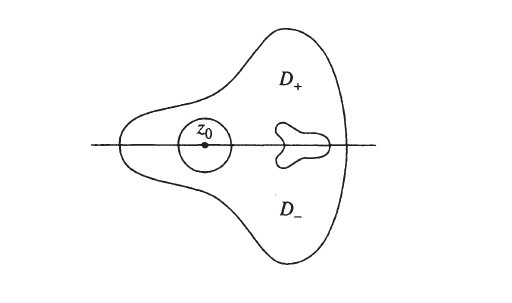
\includegraphics[width = 0.8 \textwidth]{schwarzov_princip_zrcaljenja.png}
    \end{center}
    Slika prikazuje glede na $\R$ simetrično območje $D \subseteq \C$. $D^{+}$ označuje območje na katerem harmonično funkcijo $u$ poznamo, $D^{-}$ pa območje na katerem lahko po izreku eksplicitno konstruiramo razširitev s predpisom $u(\overline{z}) = - u(z)$.
    Vodoravna črta prikazuje odsek realne osi, na kateri bodo zaradi zveznosti vrednosti trivialno poračunljive. 
    Točka $z_0$ in "majhen" disk okoli nje, nakazujeta, da se bomo dokaza lotili z lastnostjo povprečne vrednosti.


    \begin{dokaz}
        Opazimo, da je $D$ disjunktna unija $D^+$, $D^-$ in $D^0 = D \cap \mathbb{R}$.
        Hitro je razvidno, da je $u^e$ na $D$ res zvezna (na $D^+$ in $D^-$ po predpisu, na $D^0$ zaradi limite iz predpostavke izreka). 
        \newline
        Posvetimo se dokazu harmoničnosti. Ker je $u^e$ na $D$ zvezna, je po trditvi \ref{ekvhlp} dovolj pokazati, da ima $u^e$ na $D$ lastnost povprečne vrednosti.
        Na $D^+$ je $u^e$ harmonična po predpostavki, na $D^-$ pa harmoničnost hitro preverimo prek leme \ref{lemaharm}. 
        Za poljubno točko $z_0 \in D^0$, pri dovolj majhnem $r$ (tako da je $\overline{\mathbb{D}}(z_0,r) \subseteq D$) velja, da se ob računanju povprečja paroma "zrcalne" vrednosti zaradi predpisa $u(\overline{z}) = u(z)$ ravno odštejejo. 
        To pa že implicira, da je povprečje v poljubnem $z_0 \in D^0$ enako $0$ in $u^e$ tudi v $z_0 \in D^0$ izpolnjuje lastnost povprečne vrednosti.
    \end{dokaz}

    KAJ S HOLOMORFNIMI ??, DO KAM NAPREJ ??
\newpage

\bibliographystyle{siam}
\begin{thebibliography}{9}
    \bibitem{osnova}
    Theodore W. Gamelin \emph{Complex Analysis}, Springer (2001), Chapter X, str. 274 - 288

    \bibitem{mean value p}
    Weisstein, Eric W. \emph{Mean-Value Property}, v: From MathWorld--A Wolfram Web Resource, [ogled 22. 2. 2023], dostopno na \href{https://mathworld.wolfram.com/Mean-ValueProperty.html}{https://mathworld.wolfram.com/Mean-ValueProperty.html}
\end{thebibliography}

\end{document}